\documentclass[letterpaper,11pt]{article}

\usepackage[backref=section, linkbordercolor={1 1 1}, urlbordercolor={1 1 1}, citebordercolor={1 1 1}]{hyperref}
\usepackage{algorithm2e}
\usepackage{cite}
\usepackage{color}
\usepackage{float}
\usepackage{graphicx}
\usepackage{parskip}

\graphicspath{ {images/} }

\newcommand{\todo}[1]{}
\renewcommand{\todo}[1]{{\color{red} TODO:\ {#1}}}

\begin{document}

\title{Helium --- A Decentralized Wireless Network}
\author{Helium Systems, Inc}
\date{\today}
\maketitle
\thispagestyle{empty}

\begin{abstract}
The Internet of Things (IoT) is a \textdollar1.6 trillion industry, with over 8.4 billion connected devices online, and predicted to more than double over the next 2 years. All of these devices need to connect to the internet to function. However, current solutions such as cellular, WiFi, and Bluetooth are suboptimal: they are too expensive, too power hungry, or too limited in range.

Helium is a \emph{decentralized wireless network} for IoT devices that enables devices anywhere in the world to connect to the internet and geolocate themselves without the need for power-hungry satellite location hardware or expensive cellular plans. Powering the network is a blockchain with a native protocol token incentivizing a two-sided marketplace between coverage providers and coverage consumers. With the introduction of a blockchain, Helium injects decentralization into an industry currently controlled by monopolistic companies. The result is that IoT coverage becomes a utility, fueled by competition, available anywhere in the world, at a fraction of current costs.

Helium's secure and open-source primitives enable developers to build low-power, internet-connected devices quickly and cost-effectively. Helium has a wide variety of applications across industries and is the first decentralized wide area network of its kind.
\end{abstract}

\newpage

\tableofcontents
\newpage

\section{Introduction}

The world is becoming decentralized. A multitude of platforms, technologies, and services are moving from centralized proprietary systems to decentralized open ones. Peer-to-peer networks such as Napster~\cite{napster} (created by Helium founder Shawn Fanning) and BitTorrent paved the way for blockchain networks and crypto-currencies to be built. Now Bitcoin, Ethereum, and other blockchain networks have proven the utility of decentralized transaction ledgers. Existing internet services such as file storage, identity verification, and the domain name system are being replaced by modern algorithmic versions. While software-level decentralization has moved quickly, physical networks are taking longer to affect. These networks are more complicated to decentralize as often specialized and expensive hardware is required in order for these systems to function.

Helium is a wide-area wireless networking system, a blockchain and a protocol token. The blockchain runs on a new kind of proof, called \emph{Proof-of-Coverage}, where blocks are created by miners who are providing wireless network coverage in a cryptographically verified physical location and time. The Helium protocol provides a bi-directional data transfer system between wireless devices and the Internet via a network of independent providers that does not rely on a single coordinator, where: (1) devices pay to send \& receive data to the internet and geolocate themselves, (2) miners earn tokens for providing network coverage, and (3) miners earn fees from transactions, and for validating the integrity of the network.

\subsection{Philosophy}

Helium exists due to a set of core beliefs that have driven every component and the underlying purpose of the network and protocol. In this section we outline the requirements that are necessary for building a truly decentralized wireless network.

\textbf{Decentralization}. The Internet of Things (IoT) is poised to change the way we interact with the physical world and at a scale that is unprecedented, with projections of over \$11.1 trillion in economic value added in under 10 years\cite{mckinsey}. It is critical that this industry be driven forward in a truly decentralized way that allows participation from anyone, anywhere, with no arbitrary gatekeepers. There are many existing products, services and companies participating in the IoT ecosystem today, but nearly all are centralized or proprietary in some form. Some require specialized hardware available from a single vendor, some use proprietary technology, and others tightly control access to infrastructure. Helium exists to make it possible for individuals, businesses, and communities to participate and enable IoT solutions without the need to rely on or trust any external entities.

\textbf{Low Power}. Helium is focused on a specific subset of IoT---low power devices. While IoT can cover a very broad range of devices and use cases, we believe that high-power data-intensive applications are well serviced by existing network technologies such as WiFi and LTE\@. Low power wireless networking solutions are in their relative infancy, particularly those which require long range from an access point. A new class of low power wireless solutions---known as \emph{Low Power Wide Area Networks (LPWANs)}---have begun to emerge in the last several years, but are all proprietary in nature or extremely centralized in some capacity. Helium is built upon an entirely new open-source wireless networking protocol designed for IoT devices.

\textbf{Security}. IoT presents an entirely new class of security challenge. Devices can be small, portable and with limited computing power and bandwidth. Information from the physical world presents new types of attack vector that can affect more than just data. Existing IoT offerings do not typically take advantage of modern encryption, authentication and authorization security techniques. These solutions often use soft-keys easily extractable from firmware by an attacker, or communicate via networking protocols that use vulnerable pre-shared keys. We present an entirely new blockchain-based wireless security system that relies on hardware-secured key material and takes advantage of modern public key cryptography.

\textbf{Open Standards}. The evolution of networking protocols and technologies have taught us that closed ecosystems and proprietary technologies fail. Helium is built on the principles of open source and open standards technologies. There are no proprietary chipsets, obscure modulation schemes, and no closed-source software. We believe deeply in the principles of decentralization, which requires that anyone anywhere be capable of not only participating in the network, but adding to and growing it with technology of their choosing.

\textbf{Cost Effective}. Access to data from the physical world should be as cheap and cost-effective as possible. This requires creating a market-driven economic model, low network building costs, and a new type of currency suited to micro-transactions. By enabling anyone anywhere to help build and charge for this network, the participants set the prices they are willing to accept and pay. Because everything is open, there are no arbitrary points at which to extract fees and premiums.

\textbf{Developer Driven}. We believe that IoT needs developer tools that are an order of magnitude better than those currently available. Whether an individual or business, it shouldn't require deep hardware, firmware, security, and wireless expertise to get going. Moving from prototype to full product should not need a completely new effort. Helium provides a set of SDK's, reference hardware and internet applications that make sending and receiving data securely with low power hardware simple and open.

\subsection{Key Components}

Helium is built around the following key components:

\begin{enumerate}
  \item \textbf{\emph{Proof-of-Coverage}}: we present a computationally-inexpensive \emph{Proof-of-Coverage} that allows miners to prove they are capable of providing wireless network coverage. We anchor these proofs using a \emph{Proof-of-Serialization} that allows miners to prove they are accurately representing time relative to others on the network in a cryptographically secure way.

  \item \textbf{Blockchain Network}: we demonstrate an entirely new purpose-built blockchain network built to service the \emph{Wireless Protocol} and provide a system for authenticating and identifying devices, providing cryptographic guarantees of data transmission and authenticity, offer transaction primitives designed around the wireless protocol, and more.

    \item \textbf{Wireless Protocol}: we introduce a new open-source and standards-compliant wireless network protocol, called \emph{WHIP}, designed for low power devices over extremely wide areas. This protocol is designed to run on existing commodity radio chips available from dozens of manufacturers with no proprietary technologies or modulation schemes required.

    \item \textbf{Geolocation}: we outline a system for interpreting the physical \emph{geolocation} of a device using WHIP without the need for expensive and power-hungry satellite location hardware. Devices are able to make immutable, secure, and verifiable claims about their location at a given moment in time which are recorded in the blockchain.
\end{enumerate}

\subsection{System Overview}

\begin{itemize}
    \item The Helium protocol is a \emph{Decentralized Wireless Network} system built around a new wireless protocol (WHIP) on a purpose-built blockchain with a native token.
    \item Devices take the form of hardware containing a radio chip and firmware compatible with WHIP, and spend tokens by paying miners to send data to and from the internet.
    \item Miners earn tokens by providing wireless network coverage via purpose-built hardware which provides a bridge between WHIP and routers, which are internet applications.
    \item Devices store their private keys in commodity key-storage hardware and their public keys in the blockchain.
    \item Miners join the network by asserting their satellite-derived location, a special type of transaction in the blockchain, and staking a token deposit.
    \item Miners specify the price they're willing to accept for data transport and geolocation, and devices specify the price they are willing to pay. Miners are paid once they prove they have delivered data to the devices' specified router.
    \item Miners can participate in the creation of new blocks in the blockchain, for which they are rewarded newly minted Helium. A miners probability of mining the next block is approximately equal to the amount of wireless network coverage being provided.
    \item The blockchain employs \emph{Proof-of-Coverage} to guarantee that miners are correctly representing the amount of wireless network coverage they are creating.
\end{itemize}

\begin{figure}[H]
    \begin{center}
          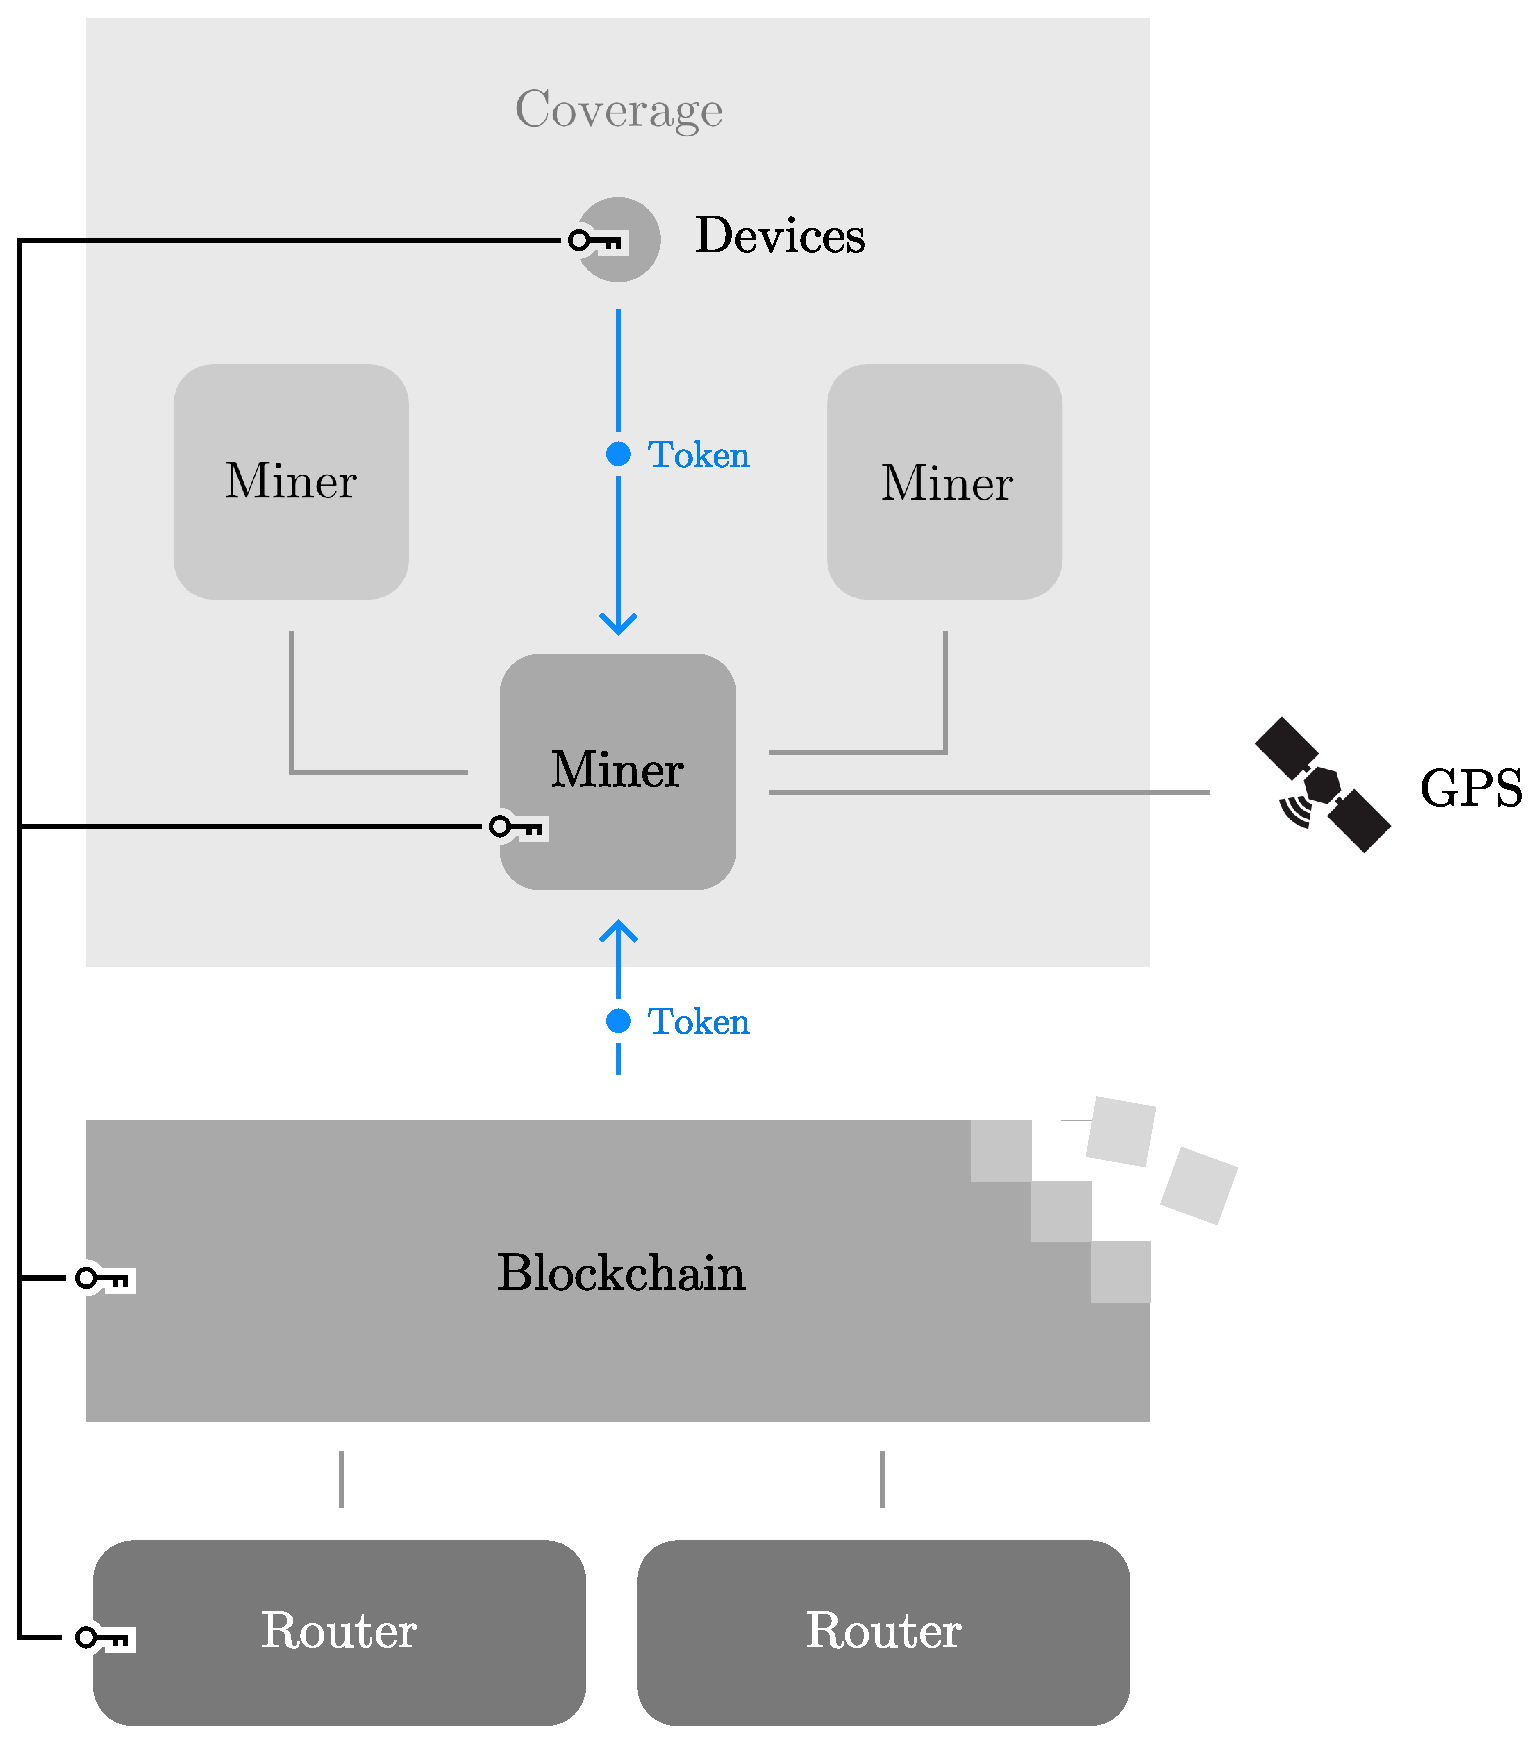
\includegraphics[width=\textwidth]{diagram1.eps}
          \caption{\emph{System Overview}}
          \label{fig:system}
     \end{center}
\end{figure}

\newpage

\section{\emph{Proof-of-Coverage} \& \emph{Proof-of-Serialization}}\label{poc}

In the Helium network, miners must prove that they are providing wireless network coverage that devices can use to communicate with the internet. Miners do this by complying with the \emph{Proof-of-Coverage} protocol which the blockchain network and other miners audit and verify. We use a \emph{Proof-of-Serialization} to ensure that miners are correctly representing their time relative to others on the network, and obtain cryptographic proof of dishonest behavior. Several components of the Helium network, such as blocks in the blockchain, use \emph{Proof-of-Serialization} as a cryptographic ``anchor'' that root those occurrences with a cryptographic time proof. With a combination of \emph{Proof-of-Coverage} and \emph{Proof-of-Serialization} we can obtain cryptographic proof of the approximate location and time of events occurring within Helium.

In this section, we outline the motivation and implementation for \emph{Proof-of-Coverage} and \emph{Proof-of-Serialization}.

\subsection{Motivation}

Most existing blockchain networks such as Bitcoin~\cite{bitcoin} and Ethereum~\cite{ethereum} use a \emph{Proof-of-Work} system that relies on an asymmetric algorithmic puzzle. These proofs are computationally difficult to generate but simple for a third party to verify. These networks achieve security by the network-wide \emph{consensus} that the amount of computing power required to generate a valid proof is expensive to forge, and as subsequent blocks are added, the increasing difficulty of the chain becoming realistically impossible to fabricate.

These computation-heavy proofs are, however, not otherwise \emph{useful} to the network. We define useful as work that is valuable to the network beyond securing the blockchain. While there have been attempts in other networks to turn mining power into something useful, such as Ethereum executing small programs, the majority of the work is not useful or reusable. The mining process is also incredibly wasteful, as the determining factor in the work is typically computational power which consumes massive amounts of power and hardware to execute.

The proofs used in Helium must be resistant to \emph{Sybil Attacks} in which dishonest miners create pseudonymous identities and use them to subvert the network and gain access to block rewards to which they should not be entitled. This is a particularly tricky attack vector to manage in a physical network like Helium. We must also be resistant to a new attack vector: \emph{Alternate Reality Attacks} exist where a dishonest group of miners can simulate that wireless network coverage exists in the physical world when it, in fact, does not. An example of this would be running the mining software on a set of virtual machines and simulating GPS coordinates and RF networking.

We later propose a consensus protocol [\ref{consensus}] that uses \emph{Proof-of-Coverage} to both secure the blockchain and provide a beneficial service to the network; providing wireless network coverage that devices can use to send data to and from the internet.

\subsection{Inspiration}

\emph{Proof-of-Coverage} (\verb|PoC|) is an innovative proof which allows miners to prove that they are providing wireless network coverage $W$ in a specific region to a challenger, $C$. \verb|PoC| is an interactive protocol where a set of targets $T_n$ assert that $W$ exists in a specific GPS location $L$ and then convinces $C$ that $T_n$ are in fact creating $W$ and that said coverage must have been created using the wireless RF network. \verb|PoC| is the first such protocol that attempts to prove the veracity of miners in a physical space, and then use it to achieve consensus on a blockchain network.

With \verb|PoC| we aim to solve the following:

\begin{itemize}
    \item Our goal is to prove that miners are operating radio frequency (RF) hardware and firmware compatible with the wireless protocol
    \item Our goal is to prove that miners are located in the geography they claim by having them communicate via RF
    \item Our goal is to correctly identify which reality is honest when there is a conflict
\end{itemize}

\emph{Proof-of-Coverage} is inspired by the \emph{Guided Tour Protocol (GTP)} which devises a system for denial of service prevention by requiring a client $c$ to request a variety of ``tour guide'' computers $G_n$ to gain access to a server $s$. The tour guides must be visited in a specific order, and a hash of data exchanged which reveals the location of the next $G_n$ in order. Only after every $G_n$ has been visited can $c$ gain access to $s$.

Once $c$ gets to the last stop of the tour, it submits evidence of the first and last stop to $s$ who can verify that the first and last stops of the tour are correct without needing to contact $G_n$, and that $c$ could only know the first and last stops if it had completed the tour correctly.

While a clever and innovative system, GTP is not directly suitable as a proof in our wireless network as radio frequency (RF) networking has limited range and therefore cannot communicate with peers everywhere on the network. We aim to construct a proof loosely based on the ideas presented in GTP, but applicable to our protocol. We refer the interested reader to~\cite{gtp} for a detailed articulation of the GTP protocol.

We combine \emph{Proof-of-Coverage} with \emph{Proof-of-Serialization}---a proof that allows miners on the network to achieve cryptographic time consensus among decentralized client. We aim to achieve rough time synchronization in a secure way that does not depend on any particular time server, and in such a way that, if a time server does misbehave, clients end up with cryptographic proof of that behavior.

\subsection{Constructing \emph{Proof-of-Coverage}}

This section describes the construction of the \emph{Proof-of-Coverage} protocol.

We aim to construct a proof that takes advantage of the following characteristics of radio frequency (RF) communication that are unique and different to internet communication:

\begin{enumerate}
    \item RF has limited physical propagation and therefore distance
    \item RF travels at the speed of light with (effectively) no latency
\end{enumerate}

Our goal is to verify whether miners in a geographical region are acting honestly and creating wireless network coverage compatible with the Helium wireless protocol (WHIP). To do this, a challenger $C$ deterministically constructs a multi-layer data packet $O$ which begins at an initial target, $T$, and is broadcast wirelessly to a set of sequential targets, $T_n$, each of which are only able to decrypt the outer-most layer of $O$ if they were the intended recipient. Each target acknowledges receipt, $R_T$, back to $C$, removes their layer of $O$, $O$\textsubscript{L-N}, and broadcasts it for receipt by the next target. Essentially, an ``envelope of envelopes'' only openable by the intended recipient.

\begin{figure}[H]
    \begin{center}
          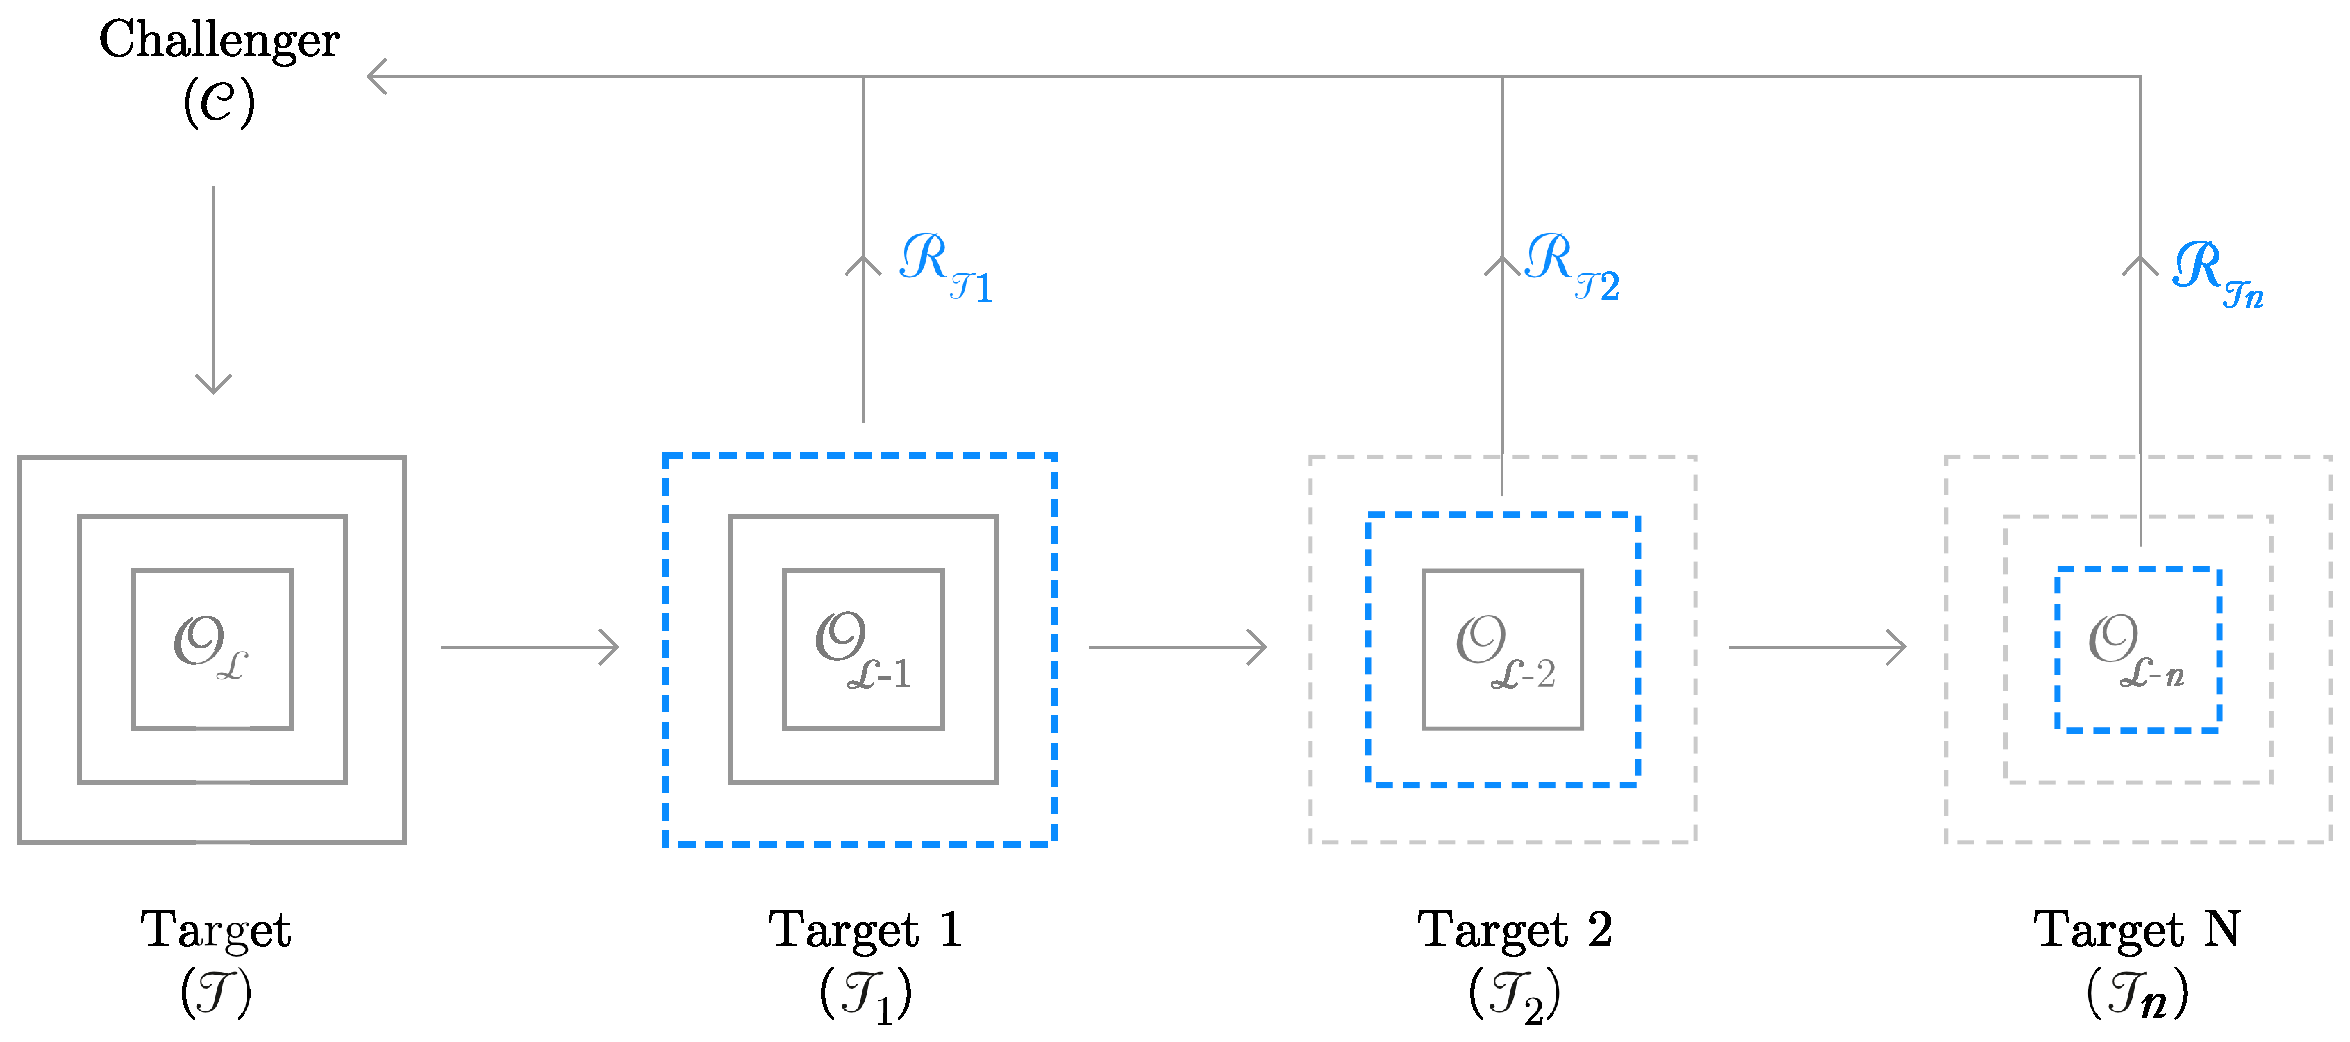
\includegraphics[width=\textwidth]{diagram2.eps}
          \caption{\emph{Multi-Layer Data Packet Deconstruction}}
          \label{fig:poc-construction}
     \end{center}
\end{figure}

\textbf{Selecting the Initial Target}. We aim to deterministically locate an initial target, $T$, for the challenger, $C$. $T$ does not need to be geographically proximate to $C$. To locate $T$, $C$ uses a \emph{consistent hash ring} $\omega$ of potential miners. $\omega$ only contains miners eligible as targets as described in [\ref{mining}], and miners are allocated portions of $\omega$ that are inversely proportional to their score, increasing the probability of potentially dishonest miners being targeted. Given that a miners score is diminishing linearly over time, it is necessary to create this inverse relationship to give low-scoring miners an opportunity to participate in the process and increase their score.

\textbf{Constructing the multi-layer challenge}. Once $T$ has been selected, $C$ must construct a multi-layer challenge, $O$. $O$ is a data packet broadcast by $T$ over the wireless network and received by geographcially proximate targets $T_n$. The number of layers of $O$ to be assembled is defined as $O_L = \log \left(T_n = \pi50^2\right)$ from the location of $T$. Each layer of $O$, $O_l$, consists of a two-tuple of $E\left(S, R\right)$, where $E$ is a secure public key encryption function, $S$ is a secret encrypted with the public key of $T_n$, and $R$ is the remainder of $O$ consisting of recursive two-tuples.

The construction logic of $O$ is as follows:

\begin{enumerate}
  \item A set of candidate $T_n$ are created within a geometric circle of an unpredictable but determinstic radius $r$ (in miles) of $T$, simply defined as $A = \pi r^2$
  \item A single $T_n$ within $A$ is psuedo-randomly selected as the first target for $O$, and designated as $T_1$
  \item A layer $O_l$ is created and $S$ is encrypted with the public key of $T_1$ retrieved from the blockchain [\ref{devices}]
  \item The next set of candidate $T_n$ are generated by inspecting a geographic area proximate to $T_1$, $A_1 = \pi r^2$
  \item A single $T_n$ within $A_1$ is again pseudo-randomly selected as the next layer of $O$, and designated as $T_2$
  \item This cycle repeats until a number of $T_n$ and $O_l$ equal to $O_L$ is reached
  \item The pseudo-random function used to determine $T_1$..$T_L$ is constructed using a hash of the current block $B_t$ as a seed, such that the selection process for $T_n$ is deterministic and therefore verifiable by others on the network
\end{enumerate}

The resulting $O$ can be visually represented as the following:

\begin{figure}[H]
    \begin{center}
          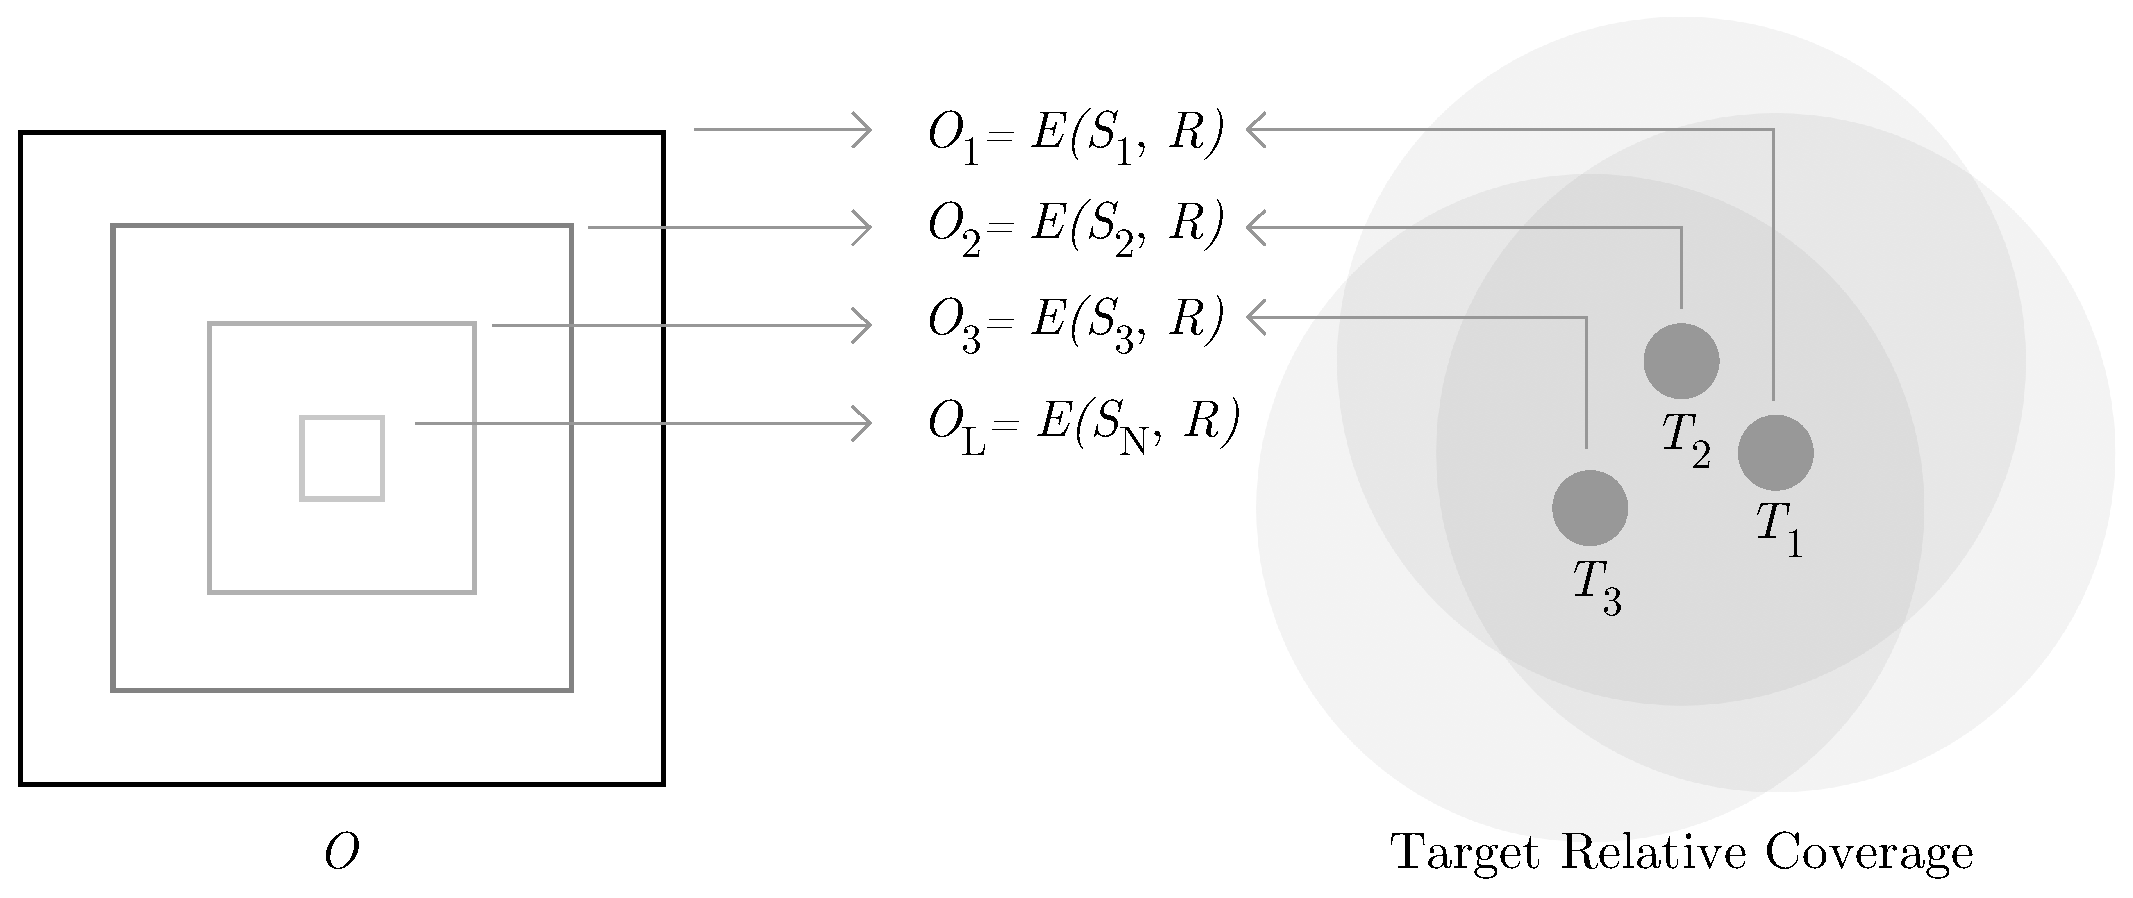
\includegraphics[width=\textwidth]{diagram3.eps}
          \caption{\emph{Construction of $O$}}
          \label{fig:onion-packet}
     \end{center}
\end{figure}

\textbf{Creating the Proof}. Once $O$ has been constructed and delivered to $T$, $T$ immediately broadcasts it. The Helium wireless protocol is not a point-to-point system, so several miners within proximity of $T$ hear $O$. As described prior, each layer $O_l$ of $O$ contains the following two-tuple: \[\mathit{E\left(S, R\right)}\] where $E$ is a secure public-key encryption function, $S$ is a secret encrypted with the public key of $T_1$, and $R$ is the remainder of $O$ consisting of recursive two-tuples. In this specific example, only the specific target $T_1$ can decrypt $S$ and send a valid receipt back to the challenger, $C$.

We describe the approximate flow of \emph{Proof-of-Coverage} creation as follows:

\begin{enumerate}
  \item $T$ receives $O$ from $C$ via the peer-to-peer internet network and immediately broadcasts it via the wireless network
  \item $T_1$ hears $O$ and attempts to decrypt the value of $S$ by using its public key $pk:\ E_{pk}\left(S\right)$
  \item If successful, $T_1$ then creates signed receipt $R_{t1} = H\left(K_s \right)$ where $H$ is a secure cryptographic hash function, and $K_S$ is $S$ signed by the private key of $T_1$
  \item $T_1$ submits $R$\textsubscript{t1} to $C$ via the peer-to-peer internet network, removes the outer most layer, and wirelessly broadcasts the remainder $O$
  \item These steps repeat for $T_2$..$T_L$, with $T_L$ being the last target constructed by $C$
\end{enumerate}

$C$ expects to hear responses from $T_n$ within a time threshold $\lambda$, otherwise, it considers the \emph{Proof-of-Coverage} to have concluded.

\begin{figure}[H]
    \begin{center}
          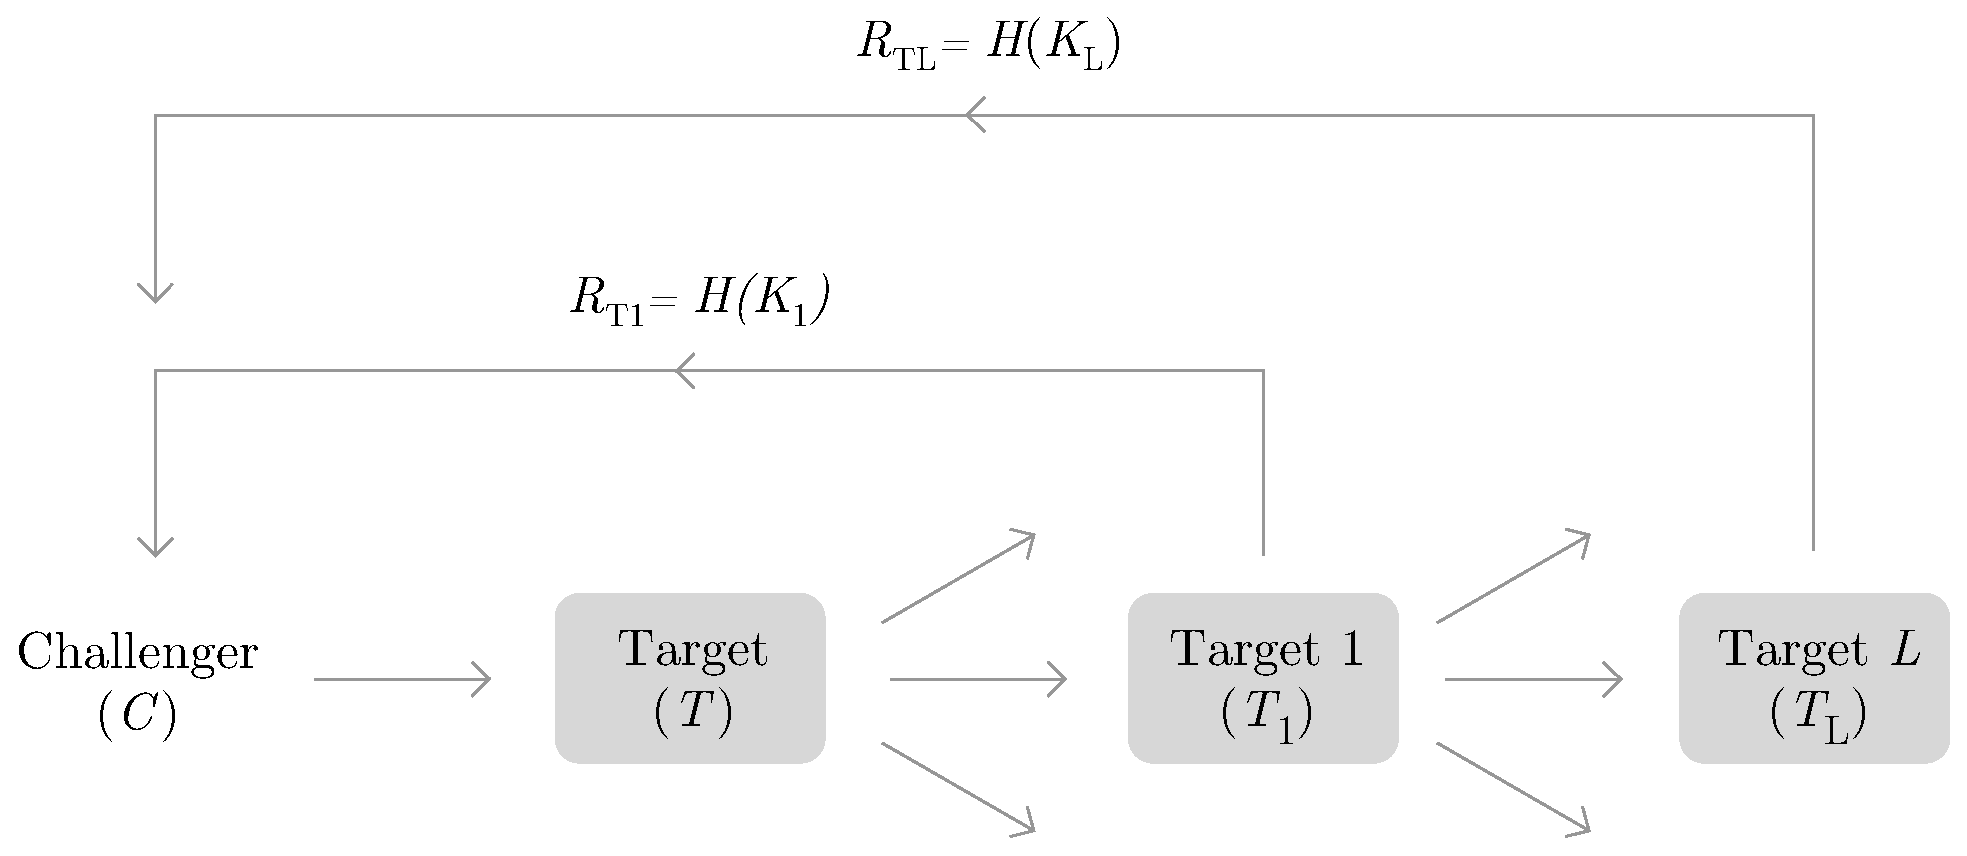
\includegraphics[width=\textwidth]{diagram4.eps}
          \caption{\emph{Proof-of-Coverage} flow}
          \label{fig:poc-flow}
     \end{center}
\end{figure}

\textbf{Scoring}\label{scores} When miners join the Helium network, they are assigned a score, $\phi$, with a value of \textbf{0.500}. This score depreciates linearly per block at a rate of $\phi = \phi - \frac{\phi}{10}$. As $\phi$ decreases the probability of the miner $M$ being the target for $C$ increases such that the network continually attempts to prove that the lowest scoring miners are acting honestly, and giving miners a reasonable chance to improve their score.

For every target $T_n$ that hears $O$ in the \emph{Proof-of-Coverage} and submits a signed receipt to $C$, $T_n$ gains a score equal to \todo{some amount relational to the previous target in the chain}.

\textbf{Verifying the Proof}. Talk here about \todo{how is PoC verified easily?}

\subsection{Constructing \emph{Proof-of-Serialization}}

This section describes the construction of the \emph{Proof-of-Serialization} protocol.

\textbf{Creating the Proof}. First, a miner $M$ pseudo-randomly picks two miners $M^1$ and $M^2$, to prove contact serialization with. It is assumed $M$ has a public key for $M^1$ and $M^2$ (otherwise $M$ should obtain it from the blockchain). $M$ then generates a salted\footnote{the salt is a 512-bit SHA of $T^t$ of $b^n R$} hash commitment $K$ called the \emph{proof-kernel}. The proof-kernel is a commitment to what claim is desired to be proven. \[\mathit{K = H\left(R || M^1 || M^2\right)}\] $M$ sends $K$ to $M^1$. $M^1$ replies with $T$, a signed message including the current time and $K$. $M$ knows that the reply from $M^1$ was not pre-generated because it includes the nonce $R$ that the $M$ generated. Because $M$ doesn't completely trust $M^1$, it asks for another time from $M^2$.

For the second request, $M$ generates a sub-proof-kernel, $L = H\left(R || T || K\right)$, and sends it to $M^2$. $M^2$ replies with $U$, a signed message including the current time and $L$. $U$ is now a proof artifact that shows that $M$ desired and then proved a serialization between $M^1$ and $M^2$. Let's assume that the times from $M^1$ and $M^2$ are significantly different. If the time from $M^2$ is before $M^1$, then $M$ has proof of misbehavior; the reply from $M^2$ implicitly shows that it was created later because of the way that $M$ constructed the nonce. If the time from $M^2$ is after, then $M$ can reverse the roles of $M^1$ and $M^2$ and repeat the process to obtain, assuming steady clocks, a misordered proof as in the other case.

With only two servers, $M$ can end up with proof that something is wrong, but no idea what the correct time is. However, with half a dozen or more independent servers, $M$ ends up with chain of proof of any server's misbehavior, signed by several others, and enough accurate replies to establish what the correct time is, $T^t$.

\textbf{Utilizing the Proven Time}. \todo{Talk here about then what? How does roughtime get used and by whom? construct this section in the same way as PoC above---professor/Rahul to complete.}

\newpage

\section{The Helium DWN}

We introduce the Helium Decentralized Wireless Network (\verb|DWN|). The \verb|DWN| provides wireless access to the internet for devices by way of multiple independent miners, and outlines a network and wireless protocol specification by which participants in the network should conform. Devices pay this network of miners for sending data to and from the internet, and miners are paid for continuously providing network coverage and delivering device data to the internet.

\subsection{Participants}

Any user can participate as a Device, a Miner, or a Router.

\begin{itemize}
    \item \emph{Devices} pay to send encrypted data to and from the internet via the \verb|DWN| using hardware compatible with the Helium wireless protocol, called \emph{WHIP} [\ref{whip}]. In geographies with a sufficient number of miners, devices can pay several miners to geolocate themselves without needing satellite location hardware. Data sent from devices is \emph{fingerprinted}, and that fingerprint stored in the blockchain.
    \item \emph{Miners} provide wireless network coverage to the network via purpose-built hardware, called gateways [\ref{gateways}], which provide a long-range bridge between WHIP and the internet. Users join the network as miners by purchasing or building a gateway that conforms to the wireless protocol, and \emph{staking} a token deposit proportional to the density of other miners operating in their area [\ref{staking}]. Miners participate in the \emph{Proof-of-Coverage} [\ref{poc}] process to prove that they are continuously providing wireless network coverage that devices can use. Miners join the network with a score [\ref{scores}] that diminishes as blocks pass without valid proofs being submitted. Miners are eligible to mine new blocks in the blockchain, and receive the block reward and transaction fees for any transactions included in the block once mined. As a miners score drops their probability of mining a block and earning the reward diminishes.
    \item \emph{Routers} are internet applications that receive encrypted device data from miners. Routers are the termination point for device data encryption. Devices record to the blockchain which routers miners should send their data, such that any gateway on the network can send any devices data to the appropriate router. Routers are responsible for confirming to the network that device data was delivered to the correct destination and that the miner should be paid for their service.
\end{itemize}

\subsection{Blockchain}

The Helium blockchain is a new type of ledger designed to provide a cost-effective way to run application logic core to the operation of a \verb|DWN|, store immutable device data fingerprints, and furnish a transaction system. We will refer to this as the Blockchain, $B$. $B$ is an immutable append-only list of transactions that achieves consensus by verifying \emph{Proofs-of-Coverage} [\ref{poc}]. Users internal and external to the \verb|DWN| have access to $B$, which is a new blockchain network built from scratch specifically for the \verb|DWN|.

$B$ consists of blocks $b_n$, which contain a header and a list of transactions. There are several kinds of transactions, outlined in [\ref{transactions}]. Although the blocks in chain can be linearly ordered, its data structure is actually a direct acyclic graph.

As in other implementations, $b_n$ consist of a hash of the previous block in the chain, a set of transactions, and a proof. At a given epoch $t$ a block $b_t$ consists of the following:

\begin{center}
    \begin{tabular}{l}
         \emph{Proof-of-Serialization} [\ref{roughtime}]\\
         Block Height \\
         Previous Block Hash \\
         Transactions \emph{1..n} Merkle Hash $T_t$ \\
         \emph{Proofs-of-Coverage} \\
         Score \\
    \end{tabular}
\end{center}

As the \emph{Proof-of-Coverage} [\ref{poc}] is valuable to the network, we store as many $b_n$ and their associated proof to $B$ as \emph{Uncle Blocks}, $U_n$. $U_n$, as described in the \emph{Greedy Heaviest-Observed Sub-Tree (GHOST)}~\cite{ghost} paper and implemented in Ethereum~\cite{ethereum}, allow a miner to earn block rewards even if their submitted block did not become the tip of the chain. $U_n$ help the winning chain accumulate `weight' in terms of both the length and quality of the chain, but also including the amount and quality of $U_n$ and their associated proofs. This means that longer chain forks, either mined maliciously or on the smaller side of a partitioned network, will not be selected over a shorter, weightier chain. This also means that valuable proofs of work aren't lost and can be used by the chain to calculate trust.

\begin{figure}[H]
    \begin{center}
          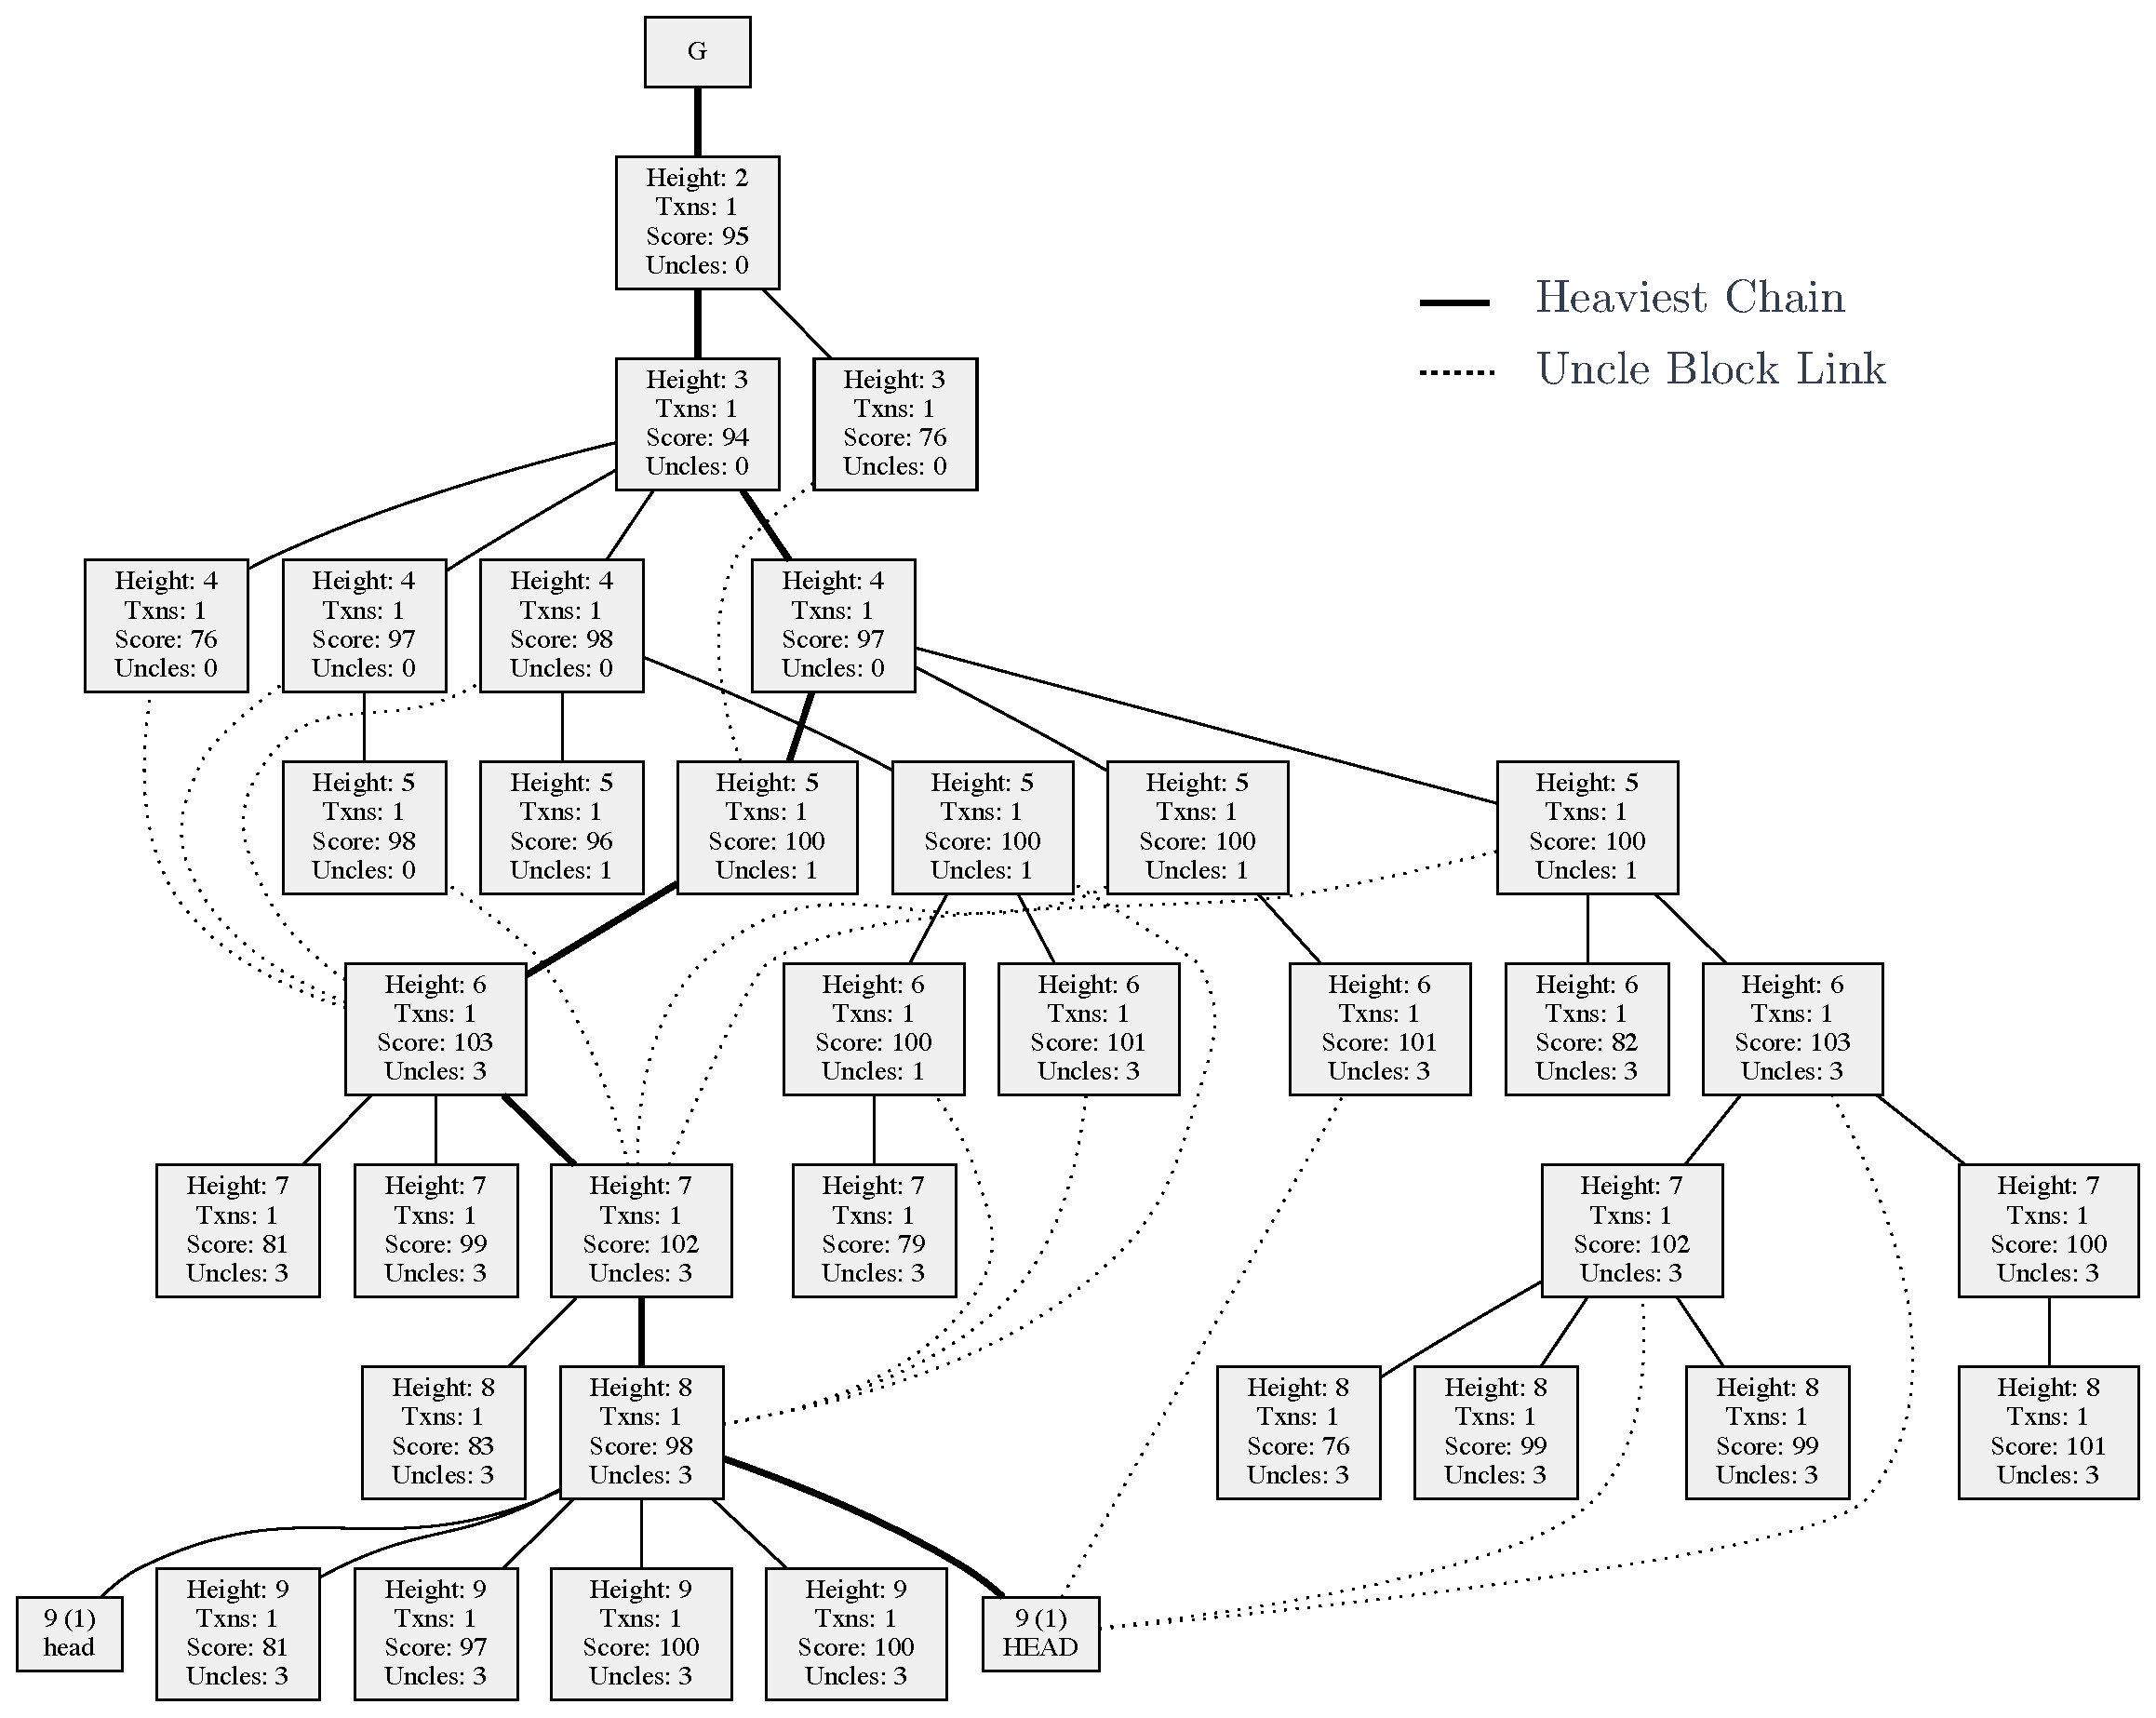
\includegraphics[width=\textwidth]{chain.eps}
          \caption{\emph{A visualization of the Helium blockchain}}
          \label{fig:chain}
     \end{center}
\end{figure}

\subsection{Protocol}

In this section we provide an overview of the Helium \verb|DWN| and the functions that Devices, Miners and Routers play in the system.

\subsubsection{Device Cycle}

We provide a brief overview of the device cycle and the functions available to devices on the network.

\begin{enumerate}
  \item \textbf{Join}: A device joins the \verb|DWN|.
  Devices join the network by \todo{professor to complete these}

  \item \textbf{Send}: A device sends data to a router on the internet, via a miner.
  Devices can send data to their specified router on the internet by paying miners Helium tokens.
  A device initiates the sending process by broadcasting a packet via the wireless protocol. When a device broadcasts a packet any miners in a reasonable geographic area hear it. Each packet header contains the devices address, and miners inspect the blockchain using this address to determine which router this devices data should be delivered to. \todo{how does the price the device is willing to pay and the miner willing to accept get determined? is it stored in the blockchain as a type of transaction?}

  \item \textbf{Receive}: A device receives data from a router on the internet, via a miner.


\end{enumerate}

\subsubsection{Miner Cycle}\label{mining}

We provide a brief overview of the mining cycle and the functions available to miners on the network.

\begin{enumerate}
  \item \textbf{Stake}: A miner joins the network and deposits a stake.
  Talk about how the stake is the ``U'' shape proportional to the density of devices in that region.

  \item \textbf{Assert Location}: A miner asserts their GPS location to the network.
  Talk about how asserting location works (it's a type of transaction? etc) and that once it's been done that miner is ready to participate in the POC process.

  \item \textbf{Challenge}: A miner begins the \emph{Proof-of-Coverage} process by becoming a Challenger.
  Talk about how this kicks off the targeting/hash ring process

  \item \textbf{Deliver}: A miner delivers data from a device to a router on the internet.
  Talk about how miners deliver data to routers and what that process looks like

  \item \textbf{Receive}: A miner receives data from a router on the internet for delivery to a device.
  Talk about how miners deliver data from routers to devices and what that process looks like

  \item \textbf{Submit}: A miner submits a new candidate block to the network containing a \emph{Proof-of-Coverage}.
  Talk about how the block submission process works, how the network verifies the block, etc

  \item \todo{are there others?}

\end{enumerate}

\subsubsection{Routing Cycle}

We provide a brief overview of the router cycle and the functions available to routers on the network.

\begin{enumerate}
  \item \todo{lay these out as above}
\end{enumerate}

\newpage

\section{Consensus Protocol}\label{consensus}

\todo{Explain how consensus works in the system, using PoC to create scores, how blocks have scores based on proofs and uncles (?) and submitting blocks that the network can somehow agree on.}

\newpage

\section{Transactions}\label{transactions}

Transactions in the Helium blockchain provide functionality that enables address-to-address transfers of Helium tokens, similar to many existing blockchain networks, but also provide a set of primitives that enable core functionality that is critical to the operation of a \verb|DWN|. In this section we address the philosophy behind our transaction system, the primitives, and the way fees on the network work.

\subsection{Philosophy}

Helium is built on the philosophy that all transactions should occur \emph{on-chain}; that is, blocks should be sized and mined with a frequency such that every transaction which occurs on the network should be stored in the blockchain rather than a \emph{side-chain} implementation such as a lightning network [\ref{lightning}] or state channel [\ref{state-channels}]. The goal of Helium is to provide internet data transport fees (the fees paid by devices to miners) that are an order of magnitude less than anything currently available for this type of service. To accomplish this goal the cost of mining must be low, blocks must be large enough to encapsulate a large number of transactions, and frequent enough that transactions are processed quickly.

Because the Helium blockchain services a specific use, the \verb|DWN|, blocks must additionally be able store fingerprints of data sent from devices along with the transaction which pays a miner for their transport service. This additional data storage would make a side-chain implementation particularly challenging, and necessitates the use of on-chain storage techniques. We believe that this holistic \emph{tamper-proof} data trail will enable entirely new use cases where the authenticity and veracity of sensor data is critical.

\subsection{Primitives in Helium}

In this section we describe the various transaction primitives.

\begin{itemize}
  \item \textbf{assert\_location}: this transaction is used by miners joining the network. Etc etc etc etc
  \item \textbf{join\_network}: devices use this\ldots
  \item \todo{marc/professor to complete these}
\end{itemize}

\subsection{Fees}

Talk about transaction vs transport and Professors IOU idea

\newpage

\section{Physical Implementation}

In addition to the blockchain network, Helium is a \emph{physical} wireless network instantiation. The participants in the network, from a physical hardware perspective, can be thought of as follows:

\textbf{Wireless Protocol (\emph{WHIP})}: The wireless network uses a new wireless protocol, called \emph{WHIP}. WHIP is a long-range low power wireless network protocol that takes advantage of commodity open-standards hardware. Hardware compatible with WHIP can communicate over many square miles in dense urban environments or hundreds of square miles in rural settings. WHIP compatible hardware can last for several years using standard batteries. WHIP uses strong public key cryptography and authentication occurs using the Helium blockchain, with all data being encrypted from end to end. WHIP is an open source networking protocol, and we have worked hard to ensure WHIP runs on hardware commonly available from dozens of vendors.

\textbf{Gateways}: Miners operate purpose-built hardware, called gateways. Gateways are physical network devices that create wireless RF coverage over wide areas and participate in the blockchain network. Gateways transmit data back and forth between routers on the internet and devices, and create \emph{Proofs-of-Coverage} for the blockchain network [\ref{poc}]. Gateways are manufactured using generally available open-standards components with no proprietary hardware. Gateways can co-operate and geolocate devices using the wireless network without any additional required hardware. Each Gateway can support hundreds of thousands of connected devices, and create coverage over many square miles. Miners operating gateways specify the price they are willing to accept for transport and geolocation services for devices.

\textbf{Devices}: Devices exist in the form of hardware products that contain a WHIP-compatible radio transceiver and communicate with gateways on the wireless network. WHIP is designed to facilitate low power data transmission and reception, so typically devices would exist in the form of battery-powered sensors that can live for several years using standard batteries (although mains-powered devices will also work quite well). Devices can exist in a variety of forms, depending on the product or use case, and a variety of transmission and reception strategies can be employed to optimize for transmission/reception frequency or battery life. It is recommended that devices use hardware-based key storage which is able to securely generate, store, and authenticate public/private key pairs without leaking the private key.

In this section we will expand on the components of the wireless network.

\subsection{Wireless Protocol (\emph{WHIP})}\label{whip}

\textbf{Motivation}: There are several Low Power Wide Area Network (LPWAN) technologies available today. This new generation of wireless technologies focus on creating extremely long range, low power internet communication for sensors and other smart devices. Typically these technologies trade speed for range, with data rates as low as 18 bits per second (bps) with range measured in miles compared to a typical WiFi network which has substantially higher data rates but range limited to only a few hundred feet. Several of these new technologies, such as LoRa [\ref{lora}] and RPMA [\ref{rpma}], have gained good traction and there are many commercial products available compatible with these systems. However, we believe that the future IoT economy should be built on non-proprietary protocols and modulation schemes, and that participants in this ecosystem should have the freedom to choose hardware and vendor. We do not consider an open alliance built on top of proprietary hardware to be an acceptable compromise. While there are many open-standards wireless networking protocols and physical layers, such as IEEE 802.15.4 [\ref{802.15.4}] used in the first generation of Helium wireless products, none meet our extremely long range and low power criteria. It is this lack of open solutions that drove the creation of a new protocol.

\textbf{Outline}: We introduce a new open-source Low Power Wide Area Network (LPWAN) protocol called \emph{WHIP}. WHIP is a highly secure, long range, low power wireless network protocol that is compatible with any Frequency Shift Keying (FSK) radio transceiver operating in the sub-GHz unlicensed frequency spectrum. Authentication with the wireless network uses modern public-key encryption and NIST P-256 ECC [\ref{ecc}] key pairs, with the public keys for all participants stored in the blockchain.

FSK is a simple modulation format that is widely supported, easy to modulate and demodulate, and has good resistance to RF noise. There are dozens of vendors implementing FSK radio transceivers compatible with WHIP, such as Texas Instruments [\ref{ti}], Microchip [\ref{microchip}], and Silicon Labs [\ref{silabs}].

WHIP is a \emph{narrowband} wireless protocol which creates hundreds of extremely small channels within the unlicensed spectrum and employs Frequency Hopping Spread Spectrum (FHSS) to pseudo-randomly hop between channels. Typically FHSS requires a complex time-synchronized system that is limited in capacity, however devices using WHIP do not need to coordinate with gateways on channel selection as gateways are capable of hearing all channels within the available spectrum at any time. We choose narrow-band to accomplish the following goals:

\begin{itemize}
    \item \textbf{Spectrum Efficiency}: it is necessary to operate within unlicensed RF spectrum very efficiently. RF is a shared, limited resource, and therefore a focus on efficiency to increase capacity and improve robustness is a must.
    \item \textbf{Co-Existence Performance}: as the number of devices and networks increases, the ability to operate in \emph{noisy} RF environments without interference is a critical consideration.
    \item \textbf{Range}: narrowband allows for extremely long-range communications, with data rates that scale both up and down depending on the density of gateways.
\end{itemize}

WHIP implements a variety of Forward Error Correction (FEC) techniques. FEC is a technique used for controlling errors in data transmission over unreliable or noisy communication channels, and can result in significantly higher radio sensitivity. FEC gives the receiver the ability to correct errors without needing to request retransmission of data, but at the cost of a fixed, higher channel bandwidth. WHIP implements these techniques at the firmware level in order to maintain hardware compatibility among multiple vendors. WHIP also supports power amplification up to regulatory limits, which vary by region.

\textbf{Implementation}: WHIP supports a number of data rates, channel bandwidths, and FEC techniques. Gateways and devices dynamically negotiate the combination of these options using a \emph{signalling packet} delivered at the lowest bandwidth and datarate to ensure the longest range for the initial communication. The signalling packet is delivered via a 4KHz channel, at a 300bps data rate, using 2-FSK modulation. This initial negotiation allows for the following eight modulation schemes:

\begin{itemize}
    \item 2-FSK
    \item 2-GFSK
    \item 4-FSK
    \item 4-GFSK
    \item 4 Reserved for future expansion
\end{itemize}

There are also eight FEC options:

\begin{itemize}
    \item None
    \item Hamming 8,4
    \item Golay 24,12
    \item Reed-Solomon + Convulational coding (the ``Voyager code'')
    \item 4 Reserved for future expansion
\end{itemize}

We also have eight combinations of data rate and deviation, which vary from 300bps to 100,000bps.

The full WHIP wireless specification will be made available by the Helium Alliance~\cite{alliance}.

\subsection{Gateways}\label{gateways}

Gateways are physical network devices operated by miners, that create wireless RF coverage over wide areas. They transmit data back and forth between routers on the Internet and devices on the network, process blockchain transactions, and create \emph{Proofs-of-Coverage} for the blockchain network [\ref{poc}]. Gateways can connect to the Internet using any TCP/IP capable backhaul, such as Ethernet, WiFi or Cellular. Each gateway contains a radio frontend capable of listening to several MHz of radio spectrum at a time, and is able to hear all network traffic transmitted within that spectrum. In this configuration modulation and demodulation is done in software, which is typically referred to as a \emph{Software Defined Radio (SDR)}. The benefit of this structure is that gateways can hear any device traffic transmitted within the frequency range, and no synchronization between the gateway and device needs to occur. This allows devices to remain inexpensive and relatively simple, and reduces wireless protocol overhead. If a miner wishes to minimize their gateway hardware costs, synchronized frequency hopping schemes are also permitted within the specification as a cheaper alternative to a more expensive radio frontend.

Gateways require a GPS or GNSS transceiver to obtain accurate position and date/time information. This satellite-derived location will be used in conjunction with other techniques to verify that a gateway is in fact providing wireless network coverage in the location it claims. Because satellite location messages are easy to fabricate and do not necessarily prove that wireless RF coverage is being created, multiple mechanisms are required to validate this work as described in more detail in [\ref{poc}].

Satellite location information is also correlated with packet arrival events to provide \emph{Time Differential of Arrival (TDoA)} location for devices if multiple gateways observe the same packet. This allows devices to physically locate themselves without requiring a GPS/GNSS transceiver, and therefore provide accurate location data at a fraction of the battery life and cost of competing methods. This method is described in detail in [\ref{geolocation}].

Helium Systems Inc.\ will make both a complete open-source reference design and a finished product available for immediate participation in the network.

\subsection{Devices}\label{devices}

A \emph{device} is any wireless hardware capable of communicating with gateways on the network. WHIP is designed to facilitate low power data transmission and reception, so typically devices would exist in the form of battery-powered sensors that can function for several years using standard batteries.

WHIP is designed such that devices can be manufactured using commodity hardware available from a wide variety of vendors, and for an extremely low-cost bill of materials (BOM). The technology in modern radio transceivers, such as the Texas Instruments CC1125 or STMicroelectronics S2-LP, enables extremely long-range network systems that can be built without the need for proprietary modulation schemes or physical layers. Some of these radios are available for around \$1 at reasonable volumes.

Each device will use the Microchip ECC508A\cite{ecc} or equivalent hardware-based key storage device, which is able to securely generate, store, and authenticate public/private \emph{NIST P-256 ECC} [\ref{ecc}] key pairs without leaking the private key. In addition, a wide array of defense mechanisms prevent logical attacks on the encrypted data between the key storage device and its host device, along with physical protections on the security device itself. Users program their key storage device as part of the onboarding process defined in the WHIP wireless specification using a simple SDK\@.

\subsection{Routers}

Routers are internet-deployed applications that receive packets from devices via gateways and route them to appropriate destinations such as an HTTP or MQTT endpoint.

There are several functions that routers serve on the network, which include:

\begin{itemize}
    \item Authenticating devices with the wireless network
    \item Receiving packets from gateways and routing them to the Internet
    \item Delivering downlink messages, including OTA updates, to devices via gateways
    \item Providing delivery confirmations to ensure transport transactions are honest
    \item Providing authentication and routing mechanisms into third-party cloud services such as Amazon AWS or Microsoft Azure
\end{itemize}

When a gateway receives a data packet from an device on the network, it will query the blockchain to determine which router to use given the devices network address. Anyone anywhere is free to host their own router and define their devices traffic to be delivered there by any gateway on the network. This allows users of the network to essentially create VPN-like functionality whereby encrypted data is delivered only to a router (or set of routers) that they specify and can optionally host themselves.

Routers can implement a system called a \emph{Channel} which handles the authentication and routing of data to a specific third party Internet application, such as Microsoft's Azure IoT Hub\cite{azure}. These channel implementations can take advantage of a devices onboard hardware security to create a secure, hardware-authenticated connection to a third party which would otherwise be difficult to implement directly on an embedded microcontroller. Helium will make available an open source reference implementation of a Channel that can be used to build additional interfaces to Internet services.

Helium Systems Inc hosts a high-availability cloud router for anyone to use, and also provides and maintains an open-source router that is available either as source code or a binary package for a variety of operating systems and distributions.

The protocol specification required for implementing a router is defined in the WHIP Wireless Specification document that will be made available by the Helium Alliance\cite{alliance}.

\subsection{Geolocation}\label{geolocation}

WHIP-compatible gateways are expected to include hardware and software to enable not only location of the gateway (via GPS/GNSS) but also hardware and software to triangulate the location of an end node. This method is typically called \emph{Time Differential of Arrival (TDoA)}. Gateways accomplish TDoA location using a radio frontend configured to output raw sample data, which can then be post-processed and compared to GPS location and time to calculate the radio packet's time of flight. With enough of these time-of-flight calculations from several gateways, the position of the device can be calculated to within several meters.

Because of the expense and power consumption of a typical GPS module, and the fact that they require a view of the sky, providing geolocation as a network service makes devices cheaper, more power efficient, and able to located accurately indoors. Additionally, because these data transmission events occur in the context of a blockchain, unforgeable cryptographic proof of location for a device can be obtained. Devices being able to prove they were in a specific place at a specific time has tremendous potential for a wide variety of IoT applications.

\begin{figure}[H]
    \begin{center}
          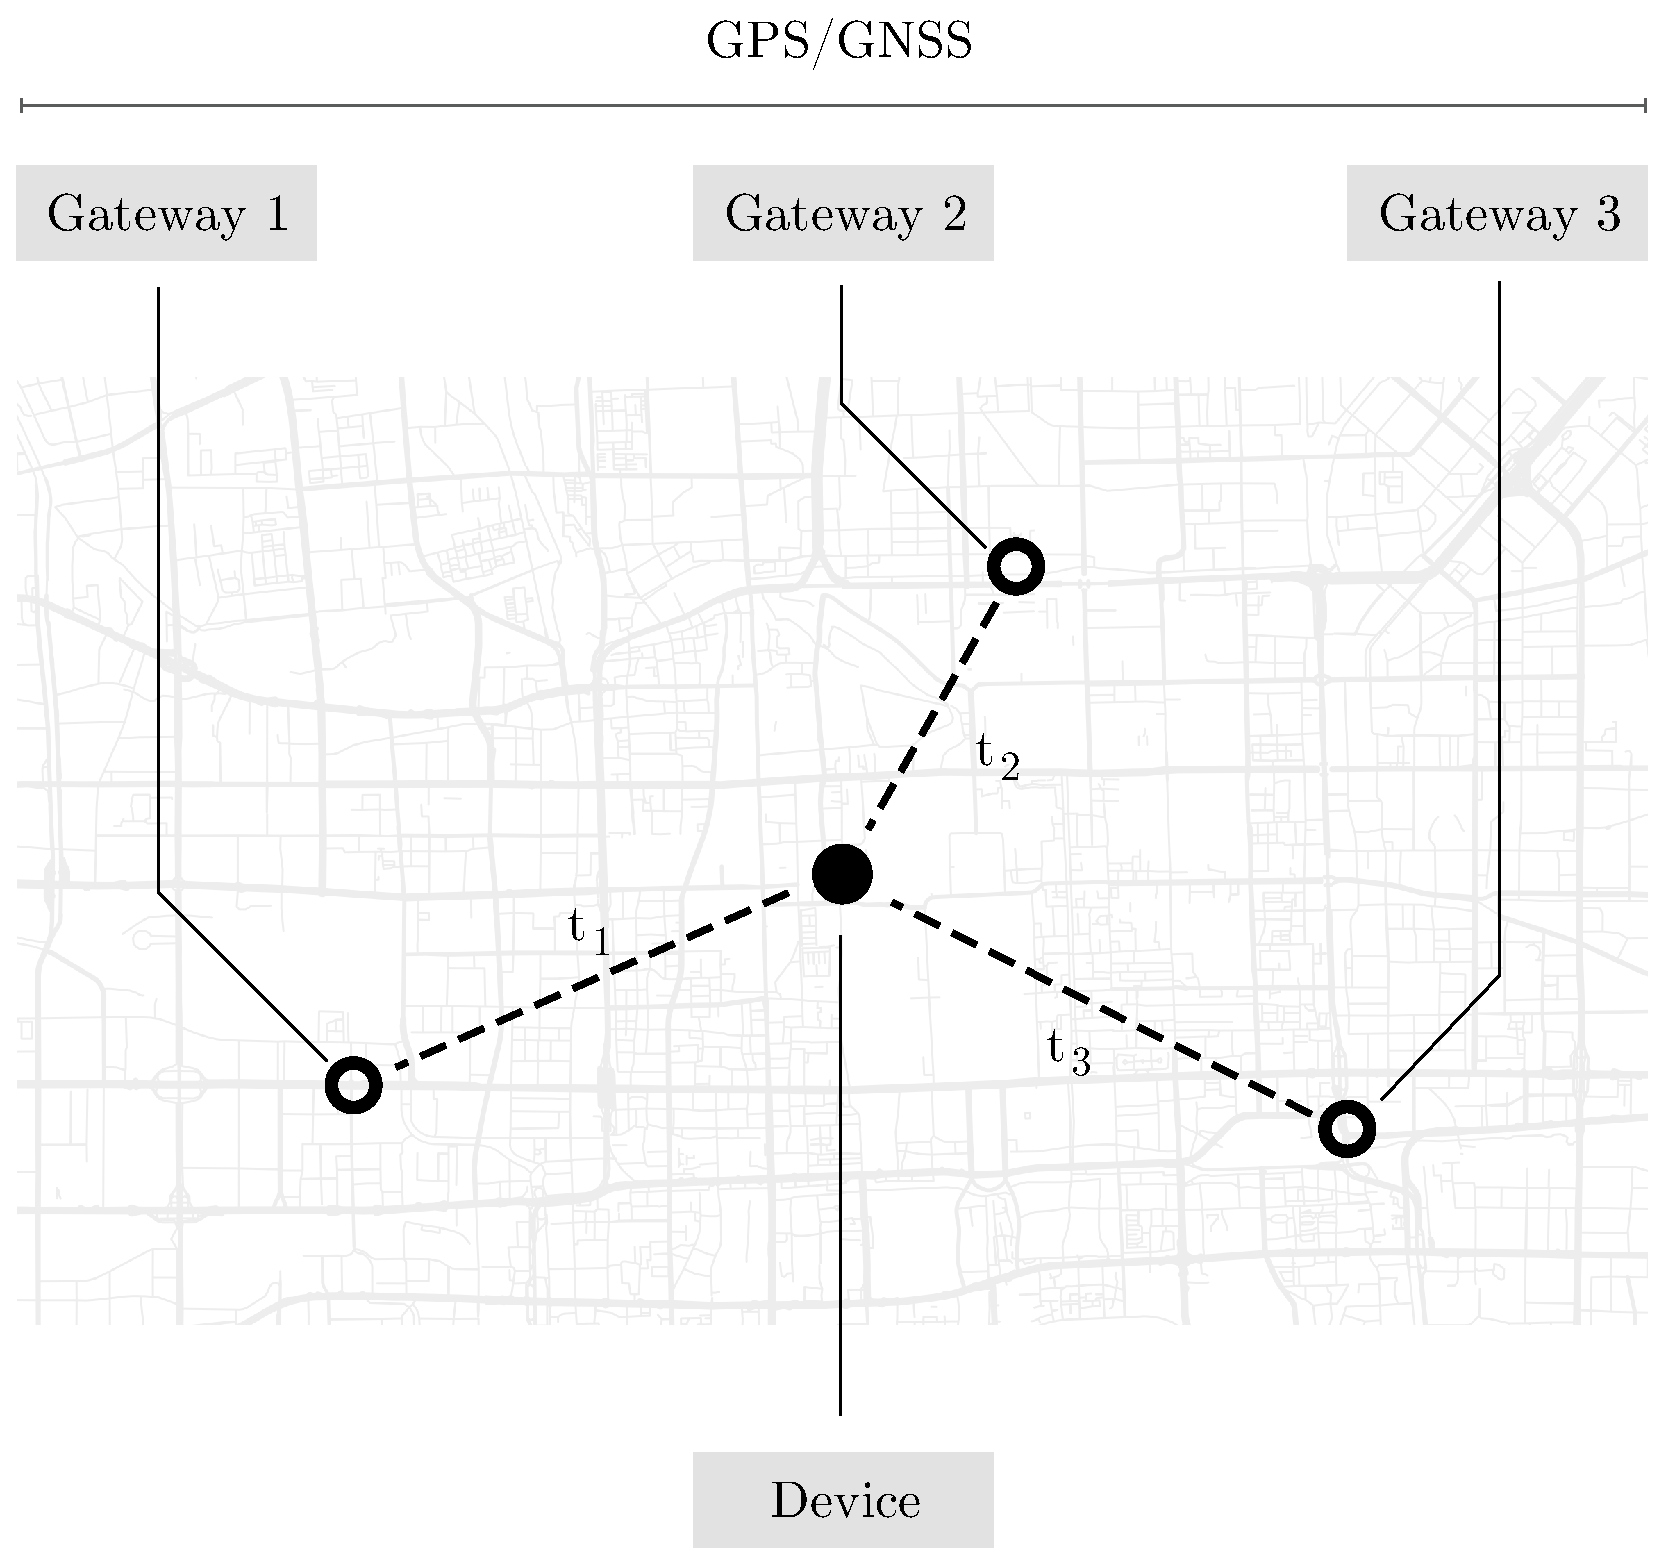
\includegraphics[scale=0.3]{tdoa.eps}
          \caption{\emph{Geolocation via TDoA}}
          \label{fig:tdoa}
     \end{center}
\end{figure}

Geolocation requires a density of gateways such that at least three gateways can hear the same packet at the same time. Because each gateway on the network is capable of listening on a wide range of radio spectrum, every gateway in range should hear the same packet with a nanosecond-level variance in the timing which can be used to solve for location via an internet application.

Gateways synchronize their clocks via GPS such that all gateways have the same nanosecond-synchronized clock source with which to timestamp packets.

We refer the interested reader to\cite{tdoa} for a detailed description of TDoA techniques.

\newpage

\section{Future Work}

Smart Contracts, better proofs, more physical layers, etc

\newpage

\section{Acknowledgements}

This document is the result of collaborative work by multiple members of the Helium team, and would not have been possible without the help, feedback, and review of the board, advisors, and collaborators of Helium. Particularly: Andrew Allen wrote the original draft of a whitepaper, laying the groundwork and thinking for this eventual project and whitepaper document; Andrew Thompson devised the critical \emph{Proof-of-Coverage} implementation, drove much of the early development and built the first simulator of this system; Marc Nijdam implemented and structured the development efforts on both the hardware and software, including implementing libp2p in Erlang; Mark Phillips added continuous review, feedback and sanity checking of this document; Jay Kickliter built the earliest hardware testing apparatus that proved much of the physical implementation was possible; Peter Main created the various illustrations and artwork, as well as providing valuable review; and Amir Haleem wrote this whitepaper based on these various concepts and works.

We would like to extend our deepest thanks to Jeremy Rubin of the MIT Digital Currency Initiative. Your earliest feedback and direction was critical to some of the design decisions and evolution of this project. We also thank the Blockchain at Berkeley team for their help and detailed review of this work.

We would also like to acknowledge many of the prior works and inventions that have allowed us to create this project, most notably Bitcoin~\cite{bitcoin} and Ethereum~\cite{ethereum}. We would also like to extend our appreciation to Protocol Labs~\cite{protocol} and Filecoin~\cite{filecoin} who demonstrated a path for regulatory-compliant sales of protocols under development and pioneered work around the SAFT, which we have borrowed from heavily.
\newpage

\begin{thebibliography}{9}

\bibitem{napster}
    Napster, \\
        \url{https://en.wikipedia.org/wiki/Napster}

\bibitem{mckinsey}
    James Manyika, Michael Chui, Peter Bisson, Jonathan Woetzel, Richard Dobbs, Jacques Bughin, Dan Aharon
        \emph{Unlocking the potential of the Internet of Things}, \\
        \url{https://www.mckinsey.com/business-functions/digital-mckinsey/our-insights/the-internet-of-things-the-value-of-digitizing-the-physical-world}

\bibitem{ghost}
    Yonatan Sompolinsky,
        \emph{Secure High-Rate Transaction Processing in Bitcoin}, \\
        \url{http://www.cs.huji.ac.il/\%7Eyoni\_sompo/pubs/15/btc\_scalability\_full.pdf}

\bibitem{ethereum}
    Vitalik Buterin,
        \emph{Ethereum},\\
        \url{http://www.ethereum.org/}

\bibitem{bitcoin}
    Satoshi Nakamoto,
        \emph{Bitcoin}, \\
        \url{https://bitcoin.org/bitcoin.pdf}

\bibitem{roughtime}
    Adam Langley, Google,
        \emph{Roughtime}, \\
        \url{https://roughtime.googlesource.com/roughtime}

\bibitem{gtp}
    Mehmud Abliz, Taieb Znati,
        \emph{A Guided Tour Puzzle for Denial of Service Prevention}, \\
        \url{http://citeseerx.ist.psu.edu/viewdoc/download?doi=10.1.1.596.9426&rep=rep1&type=pdf}

\bibitem{tdoa}
    Regina Kaune, Julian Horst, Wolfgang Koch
        \emph{Accuracy Analysis for TDOA Localization in Sensor Networks}, \\
        \url{http://fusion.isif.org/proceedings/Fusion_2011/data/papers/217.pdf}

\bibitem{ecc}
    Microchip
        \emph{ATECC508A}, \\
        \url{http://www.microchip.com/wwwproducts/en/ATECC508A}

\bibitem{azure}
    Microsoft
        \emph{Azure IoT Hub}, \\
        \url{https://azure.microsoft.com/en-us/services/iot-hub/}

\bibitem{merkle}
    Wikipedia
        \emph{Merkle Trees}, \\
        \url{https://en.wikipedia.org/wiki/Merkle_tree}

\bibitem{alliance}
    Helium Alliance, \\
        \url{https://helium-alliance.org}

\bibitem{protocol}
    Protocol Labs, \\
        \url{https://protocol.ai}

\bibitem{filecoin}
    Filecoin, \\
        \url{https://filecoin.io}

\end{thebibliography}

\end{document}
